\def\year{2014}
%File: formatting-instruction.tex
\documentclass[letterpaper]{article}
\usepackage{aaai}
\usepackage{times}
\usepackage{helvet}
\usepackage{courier}
\usepackage[utf8]{inputenc}
\usepackage{fancyvrb}
\usepackage{listings}
\lstset {
    mathescape,
    frame=none
}
\usepackage{graphicx}
\graphicspath{ {img/} }
\frenchspacing
\setlength{\pdfpagewidth}{8.5in}
\setlength{\pdfpageheight}{11in}
\pdfinfo{
/Title (prendizagem por Reforço Active Temporal Difference Learning)
/Author (Guilherme de M. M. Taschetto, João Pedro Chagas)}
\setcounter{secnumdepth}{0}
\begin{document}

\title{Aprendizagem por Reforço\\Active Temporal Difference Learning}
\author{Guilherme de M. M. Taschetto, João Pedro Chagas\\
Acadêmicos da Faculdade de Informática da\\
Pontifícia Universidade Católica do Rio Grande do Sul\\
Av. Ipiranga, 6681\\
Porto Alegre, Rio Grande do Sul 90619-900}

\maketitle
\begin{abstract}
Este artigo tem por objetivo apresentar uma aplicação de um algoritmo de Aprenziado por Reforço
no contexto de um labirinto onde o personagem Link deve encontrar um baú através de um caminho
de forma a maximizar a recompensa final obtida. Além dos argumentos para a escolha do algoritmo,
são apresentados detalhes da implementação e apresentação e análise dos resultados obtidos.
\end{abstract}

\section{Introdução}

Nosso agente, Link, tem por objetivo caminhar por um labirinto e chegar ao final (marcado pela
presença de um baú) maximizando a recompensa obtida. A recompensa pode ser representada da
seguinte forma:

\begin{itemize}
\item +50 ao encontrar o baú;
\item +5 ao encontrar uma \textit{rupee}\footnote{Uma espécie de pedra preciosa.};
\item -0.1 ao caminhar ou dar de cada com uma parede.
\end{itemize}

Além disso, ao tentar mover-se em uma direção X, Link pode...

\begin{itemize}
\item avançar na direção X, com 70\% de chances que isso ocorra;
\item avançar em uma direção perpendicular à X, com 30\% de chances que isso ocorra - sendo 15\%
de chance para cada lado.
\end{itemize}

É neste contexto que desejamos aplicar um algoritmo de Aprendizado por Reforço. Através de
sucessivas experiências - ou seja, andar e conhecer o labirinto e suas caracterísricas - Link
deverá ser capaz de realizar aprimoraramentos o resultado obtido por seu caminhamento - ou seja,
aprender com a sua própria experiência.

\section{Escolha do Algoritmo}

Dentre as opções possíveis de algoritmos de Aprendizado por Reforço optamos pelo
\textit{Active TD Learning}\footnote{\textit{Active Temporal Difference Learning}, ou Aprendizado
Ativo por Diferença Temporal.}. Os principais fatores que levaram à escolha forama maior
simplicidade de compreensão e implementação, além de apresentar uma maior precisão ao ser
comparado com algoritmos similares, já que se baseia em ajustar as utilidades dos estados para
que o mais próximo possível do resultado esperado (após a convergência).

\section{Descrição do Algoritmo}

O \textit{ATDLR} pode ser dividido em duas grandes partes:

\begin{description}
\item[Atualização das Utilidades] Etapa na qual o agente transita no espaço de estados,
seguindo uma política $\pi$, e é feito o recálculo das utilidades dos estados.
\item[Atualização da Política] Etapa na qual é criada uma nova política baseada nos
novos valores de utilidades.
\end{description}

\subsection{Atualização das Utilidades}

Esta etapa faz uso de alguns artefatos. São eles:

\begin{description}
\item[$\pi$] Uma política inicial qualquer.
\item[$U(s)$] Utilidade para o estado $s$ (inicialmente $0$).
\item[$N(s)$] Número de visitas ao estado $s$.
\item[$\alpha$] Taxa de aprendizado (normalmente $1/(N(s)+1)$).
\end{description}

O algoritmo em si é descrito pelo seguinte pseudo-código:

\begin{lstlisting}
$if\ s\prime\ is\ new\ then\ U[s\prime]\ \leftarrow\ r\prime$
$if\ s\ is\ not\ null\ then$
$\ \ \ \ increment\ N_s[s]$
$\ \ \ \ U[s]\ \leftarrow\ U[s]\ +\ \alpha (N_s[s])(r\ +\ \gamma U[s]\ -\ U[s])$
\end{lstlisting}

Em linhas gerais, o algoritmo transita entre os estados utilizando a política $\pi$. Em cada
transição de estados, i. e. $s \rightarrow s\prime$, o algoritmo é executado. Descritivamente,
o algoritmo verifica se o estado atingido nunca havia sido atingido antes - em caso positivo,
a utilidade do estado é a própria recompensa imediata do estado. E, caso o estado anterior seja
válido (ou seja, não nulo), é feito o incremento no contador de visitas daquele estado e
atualizada a utilidade do mesmo seguindo a fórmula do algoritmo.

Entretanto, para tornar o algoritmo mais flexível e fazer com que ele busque por novos caminhos
(que podem ser benéficos), é adicionada uma função de exploração:

\[U[s]\ \leftarrow\ U[s]\ +\ \alpha (N_s[s])(r\ +\ \gamma U[s]\ -\ f(U[s],\ N[s]))\]

Sem a função de exploração a utilidade leva a recompensas dos estados colaboram majoritariamente
para a utilidade do mesmo. Isto faz com que o algoritmo fique muito ``preso'' aos números e acabe
não explorando o espaço de estados suficientemente - por exemplo, por outras recompensas positivas.
Esta diferença entre ``exploitation'' (seguir as utilidades calculadas) e ``exploration'' (ser um
pouco aventureiro para, quem sabe, encontrar algo de positivo).

\subsection{Atualização da Política}

Para tornar a atualização das utilidades dos estados algo útil deve ser gerada uma nova política
com base nestes valores. Uma política compreende um mapeamento $\pi(s) \rightarrow Action$, ou
seja, a política define uma ação para cada estado.

O \textit{ATDLR} define que, de tempos em tempos, a política deve ser recalculada. Para isto, é
necessário realizar o processamento de um MDP\footnote{\textit{Markov Decision Process}, ou
Processo de Decisão de Markov.} A nova política para um estado $s$ se dá por:

\[\pi(s) = arg\ max_a \sum\limits_{s\prime} P(s\prime|s,a) * U(s\prime)\]

Ou seja, a política do estado $s$ é a ação que maximiza a utilidade esperada. A função $P(s\prime|s,a)$
traduz, na fórmula, as probabilidades descritas no início deste relatório (70\% + 15\% + 15\%).

\section{Descrição da Implementação}

Em nossa implementação criamos uma classe \texttt{Tdlr} para servir como um \textit{façade} para
as diferentes partes do algoritmo. O algoritmo pode ser configurado pelos seguintes parâmetros:

\begin{description}
  \item[$float\ gamma\ =\ .9f;$] \hfill \\
  Fator utilizado para acelerar a convergência.
  \item[$int\ policySteps\ =\ 1;$] \hfill \\
  De quantos em quantos passos a política será recalculada.
  \item[$int\ explorationThreshold\ =\ 20;$] \hfill \\
  O limiar de exploração utilizado pela função de exploração.
  \item[$float\ maximumReward\ =\ 55;$] \hfill \\
  A recompensa máxima, também utilizada pela função de exploração.

\end{description}

\subsection{Estruturas de Dados}

\begin{description}
\item[$\pi$] \hfill \\ $HashMap$ encapsulado pela classe $DynamicPolicy$.
\item[$U(s)$] \hfill \\ $HashMap<State, Float> U$.
\item[$N(s)$] \hfill \\ $HashMap<State, Integer> N$.
\item[$\alpha$] \hfill \\ Método $Tdlr\#alpha(int n)$.
\end{description}

\subsection{Interface Pública}

\begin{description}
\item[$Tdlr\#updateUtilities(s\prime,\ s)$] \hfill\\
  Método que executa a parte I do algoritmo, atualizando as utilidades dos estados recebidos
  nos parâmetros.
\item[$Tdlr\#updatePolicy(tileMap, currentPolicy)$] \hfill\\
  Método que atualiza a política. O parâmetro $tileMap$ é utilizado para saber o tamanho do
  labirinto. O parâmetro $currentPolicy$ contém a política atual. Internamente, o método utiliza
  um contador parametrizável para realizar o cálculo a cada $policySteps$ passos.
\end{description}

A implementação chama o método $updateUtilities(s\prime,\ s)$ a cada passo dado por Link,
recalculando as utilidades dos estados envolvidos no passo. O método
$updatePolicy(tileMap, currentPolicy)$ também é chamado a cada passo, porém uma nova política
só é efetivamente gerada após $policySteps$ passos. Enquanto isso, o método retorna a própria
$currentPolicy$.

\subsection{Outras Considerações}

Além da nossa implementação, alguns ajustes tiveram que ser feitos no código fornecido pelo
professor para que as coisas funcionassem de forma mais satisfatória. Foram elas:

\begin{description}
\item[$State\#equals$] \hfill \\Removido a validação da propriedade $reward$ para dizer que dois objetos $State$ são iguais. Isto causava conflitos nos HashMaps que utilizam o $equals$ em casos de \textit{bucket conflicts}.
\item[$Player\#computeNextMove$] \hfill \\ Duas aterações foram feitas aqui:
  \begin{itemize}
  \item Adicionada validação para que Link pegue o \textit{rupee} somente uma vez (do contrário ele ficaria pegando infinitos \textit{rupees} para recompensa infinita).
  \item Havia um bug na construção do estado $current$, onde os parâmetros $x$ e $y$ estavam trocados.
  \end{itemize}
\end{description}

\section{Resultados}

\begin{figure}[ht]
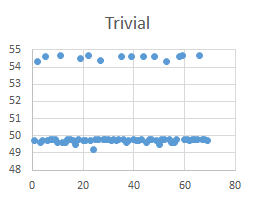
\includegraphics{trivial}\\
\centering
\end{figure}

Para o mapa $trivial$ não foi possível observar o efeito do aprendizado.

\begin{figure}[ht]
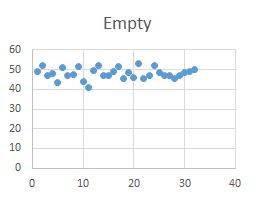
\includegraphics{empty}\\
\centering
\end{figure}

Para o mapa $empty$ é possível observar que os resultados começam a ficar uniformes após cerca de 25 execuções e à partir daí entram em uma leve crescente.

\begin{figure}[ht]
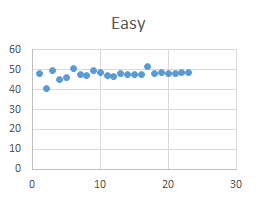
\includegraphics{easy}
\centering
\end{figure}

Para o mapa $easy$ é possível observar que os resultados começam a ficar uniformes após cerca de 10 execuções e à partir daí entram em uma leve crescente.

\subsection{Bugs e Fracassos}

Infelizmente, nosso algoritmo apresentou falhas que não conseguimos identificar mesmo após muito esforço e depuração. Em diversas simulações houve casos
em que Link ficava ``preso'' em um ciclo infinito entre dois estados ($UP \rightarrow DOWN \rightarrow UP \rightarrow \ldots$). Verificamos os valores de
utilidades e concluímos que a política estava sendo calculada corretamente, pois as ações indicavam o caminho mais vantajoso naquela redondeza e o limiar
de exploração já havia chegado ao fim. Apesar de muito quebrar a cabeça, não conseguimos bolar um artifício para evitar o surgimento deste problema/bug.

Este fato foi muito mais acentuado no mapa $medium$. Após 2 ou 3 execuções completas, o algoritmo invariavelmente ficava preso em um caso como este. Por
isto a ausência de resultados com este mapa.

\section{Conclusão}

Durante a da implementação do algoritmo foram encontradas diversas dificuldades para que o algoritmo executasse da maneira correta. Dentre essas dificuldades
podemos listar alguns pequenos bugs no código fornecido que tomaram bastante tempo para descobrí-los; a dificuldade monstruosa de debugar o código, já que
tendo dados em $hashes$ diferentes que são atualizados dinamicamente várias vezes seguidas é muito difícil de acompanhar; a falta de exemplos práticos disponíveis
na literatura e na web (embora os algoritmos estivessem bem documentados na bibliografia da disciplina).

Entretanto, a realização do trabalho foi uma ótima forma de experimentar na prática algoritmos de Aprendizado de Máquina e a resolução de MDPs. Estas duas
ferramentas associadas podem realizar façanhas incríveis no mundo da Inteligência Artificial e em diversos outros campos da ciência e tecnologia.

Na execução deste trabalho, mesmo com algumas dificuldades encontradas já descritas anteriormente, foi possível perceber que certamente utilizando a implementação de um algorimo de aprendizagem por reforço, para a exploração
de um espaço de estados, é muito mais eficiente do que muitos algoritmos conhecidos tendo em vista que é inserida
uma inteligência nova no algoritmo, que o torna capaz de realizar decisões a partidar uma exploração correta do
ambiente no qual ele está frequentando e possível perceber que mesmo com grandes opções de caminhos que podem ser tomados, utilizando os ferramentas propostos é possível facilitar a decisão do agente e fazer com que convirja para uma média de bons resultados o mais rápido possível 


\end{document}